\mainmatter%
\setcounter{page}{1}

\lectureseries[\course]{\course}

\auth[\lecAuth]{Lecturer: \lecAuth\\ Scribe: \scribe}
\date{October 1, 2009}

\setaddress%

% the following hack starts the lecture numbering at 2
\setcounter{lecture}{1}
\setcounter{chapter}{1}

\lecture{Probability Review II}

\section{Multiple Random Variables}
Start with a pair of RVs that are put together where $(X,Y):(\Omega,\Sigma) \to (\mathbb{R}^m\times \mathbb{R}^n,B)$.
Note that $X$ and $Y$ are in some sample space.
In the remainder of this course we will assume that probability density functions exist.

\begin{theorem}
\label{th:02expectationlo}
The expectation operator $E$ is a linear operator.

If $A\in k\times m$, $B\in k\times n$, then $E[AX+BY]=AE[X]+BE[Y]$.
\end{theorem}
\begin{proof}
This proof is for the one dimensional case.
\begin{align*}
E[AX+BY] &= \int_{\mathbb{R}\times\mathbb{R}}(AX+BY)p(x,y)dxdy \\
&= \int_{\mathbb{R}}\int_{\mathbb{R}}AXp(x,y)dxdy + \int_{\mathbb{R}}\int_{\mathbb{R}}BYp(x,y)dxdy \\
&= A\int_{\mathbb{R}}\int_{\mathbb{R}}Xp(x,y)dxdy + B\int_{\mathbb{R}}\int_{\mathbb{R}}Yp(x,y)dxdy \\
&= AE[X] + BE[Y]
\end{align*}
\end{proof}

Let $X\sim N(m\in\mathbb{R}^n,C)$, then
$$p(x)=\frac{1}{{(2\pi)}^{n/2}|C|^{1/2}}e^{\left[-\frac{1}{2}{(x-m)}^T C^{-1}(x-m)\right]}$$
Let $k=\frac{1}{{(2\pi)}^{n/2}|C|^{1/2}}$.

\begin{theorem}
\label{th:02mean}
\begin{align}
\label{eq:02mean}
E[x] = m \\
\label{eq:02covariance}
E[(x-m){(x-m)}^T] = C
\end{align}
\end{theorem}
\begin{proof}
The proof for (\ref{eq:02covariance}) follows Theorem~\ref{th:02covariance} later in this lecture.
This proof is for the one dimensional case of (\ref{eq:02mean}).
Let $C=\sigma^2$, $x=m+(x-m)$, $f(y)=yke^{-\frac{1}{2\sigma^2}y^2}$

\begin{align*}
E[x] &= \int xke^{-\frac{1}{2\sigma^2}{(x-m)}^2}dx \\
&= \int mke^{-\frac{1}{2\sigma^2}{(x-m)}^2}dx + \int(x-m)ke^{-\frac{1}{2\sigma^2}{(x-m)}^2}dx \\
&= m \cdot 1 + \int_{-\infty}^\infty yke^{-\frac{1}{2\sigma^2}y^2}dy \\
&= m + 0 = m
\end{align*}
In the third equality a change of variables was used where $y=x-m$ and $dy=dx$.
Then, since $f(y)$ is an odd function ($f(y)=-f(-y)$, see Figure~\ref{fig:02oddFunction}) and $\int_{-\infty}^\infty|f(y)|dy < \infty$ then that term is equal to zero.
\end{proof}

\begin{figure}[ht!]
\centering
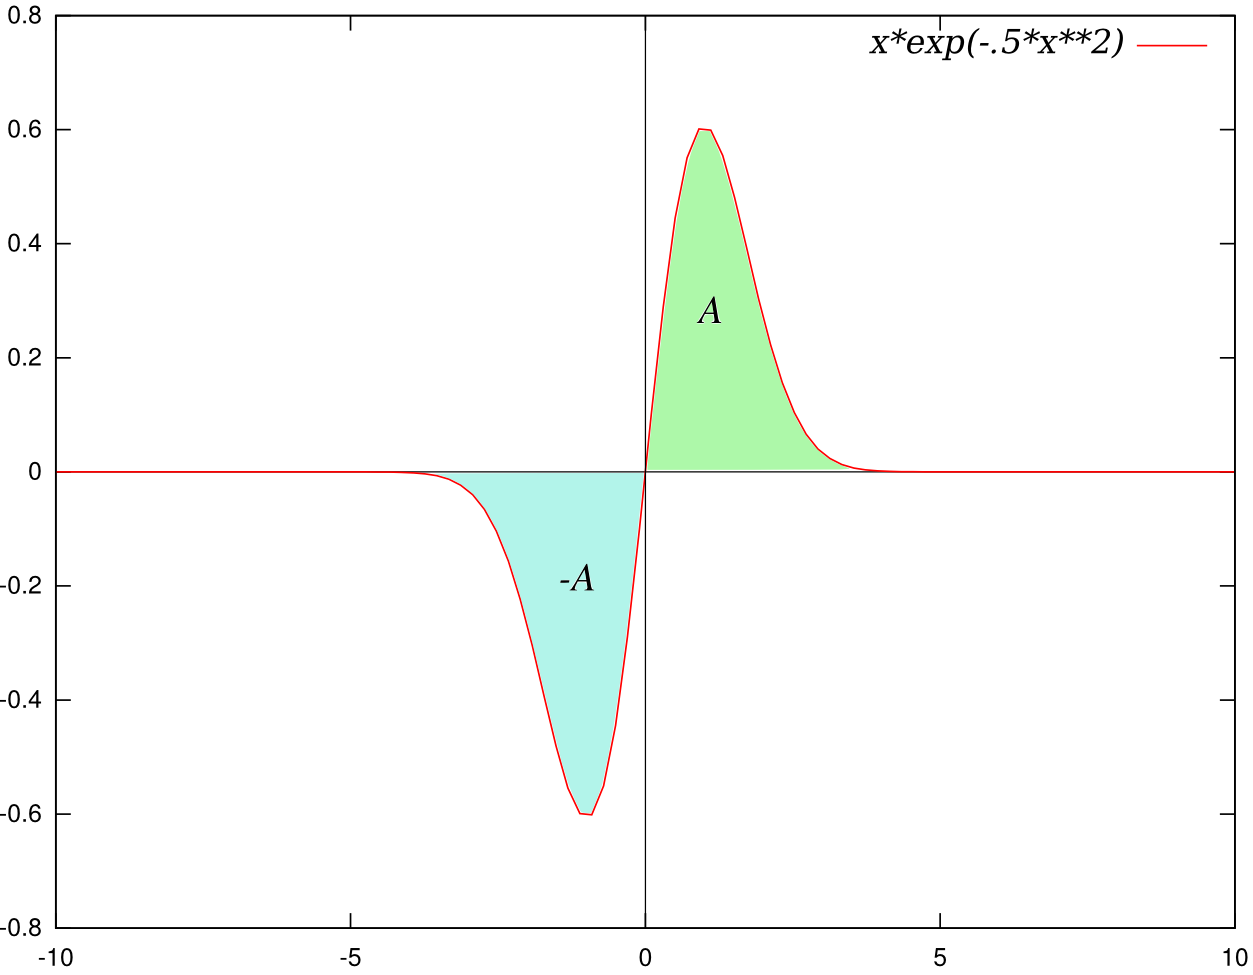
\includegraphics[width=.5\textwidth]{images/02oddFunction}
\caption{An odd function, where the integral is zero because the areas $-A$ and $A$ to the left and right of the origin are symmetric and cancel each other out.}
\label{fig:02oddFunction}
\end{figure}

\begin{theorem}
If $X$ and $Y$ are normal RVs, then $AX+BY$ is also a normal RV\@.
\end{theorem}

\begin{example}
Let $(X(\omega),Y(\omega)) \in \mathbb{R}^2$ so that $X$ and $Y$ are scalars and let $Z=(X,Y)$.
Recall that
\begin{align*}
F(x,y) &= P(X\leq x, Y\leq y) \\
&= P(\lbrace \omega\in\Omega | X(\omega)\leq x, Y(\omega)\leq y\rbrace) \\
&= \int_{-\infty}^y\int_{-\infty}^x p(x,y)dxdy
\end{align*}

Then let $A=\lbrace(x,y) | x\in(a_1,b_1], y\in(-\infty,b_2]\rbrace$, $B=\lbrace(~) | x\leq a_1, y\leq b_2\rbrace$ and $C=\lbrace(~)|x\leq b_1, y\leq b_2\rbrace$, as shown in Figure~\ref{fig:02twoSets}.% chktex 9
This gives $C=A\cup B$, $A\cap B=\emptyset$.
$$Z^{-1}(A)\cap Z^{-1}(B) = \emptyset$$
Since $P$ is a probability measure
$$P(Z^{-1}(C)) = P(Z^{-1}(A\cup B)) = P(Z^{-1}(A))+P(Z^{-1}(B))$$
or
$$P(Z^{-1}(A))=P(Z^{-1}(C))-P(Z^{-1}(B))$$
This all leads to
\begin{align*}
C &= F(b_1,b_2) - F(a_1,b_2) \\
&= \int_{-\infty}^{b_1}\int_{-\infty}^{b_2} p(x,y)dxdy - \int_{-\infty}^{b_1}\int_{-\infty}^{a_1}p(x,y)dxdy \\
&= \int_{-\infty}^{b_2}\int_{a_1}^{b_1} p(x,y)dxdy
\end{align*}
$\lozenge$
\end{example}

\begin{figure}[ht!]
\centering
\includegraphics[width=.35\textwidth]{images/02twoSets}
\caption{Two sets, $A$ and $B$, showing the distributions of RVs.}
\label{fig:02twoSets}
\end{figure}

\begin{theorem}
For any measurable $A\subseteq\mathbb{R}^n$ then
$$P(x\in A)=P(X^{-1}(A)) = \int_A p(x)dx$$
\end{theorem}

\section{Independence}
\begin{definition}
The random variables $X$ and $Y$ are independent if
\begin{align*}
P(X\in A, Y\in B) &= P(X^{-1}(A) \cap Y^{-1}(B)) \\
&= P(X^{-1}(A)) P(Y^{-1}(B)) \\
&= P(X\in A) \cdot P(Y\in B)
\end{align*}
\end{definition}

\begin{example}
Using the uniform system shown in Figure~\ref{fig:02unitSquare} we have
$$p(x,y) = \begin{cases} 1, & x\in[0,1],y\in[0,1] \\ 0, & \text{elsewhere} \end{cases}$$
Let $A,B\subseteq\mathbb{R}$, then
\begin{align*}
P(X^{-1}(A) \cap Y^{-1}(B)) &= {\int\int}_{A\times B} p(x,y)dydx \\
&= \int_{A\cap[0,1]}\int_{B\cap[0,1]} 1 dydx \\
&= \int_{B\cap[0,1]}dy \int_{A\cap[0,1]}dx \\
&= \int_{B\cap[0,1]}\int_{[0,1]}dxdy \cdot \int_{A\cap[0,1]}\int_{[0,1]}dydx \\
&= \int_{\mathbb{R}\times B}p(x,y)dydx \cdot \int_{\mathbb{R}\times A}p(x,y)dydx \\
&= P(Y^{-1}(B)) P(X^{-1}(A))
\end{align*}
$\lozenge$
\end{example}

\begin{figure}[ht!]
\centering
\includegraphics[width=.3\textwidth]{images/02unitSquare}
\caption{Unit square.}
\label{fig:02unitSquare}
\end{figure}

\begin{example}
Let $A=[0,\frac{1}{2}]$ and $B=[0,\frac{1}{2}]$, as shown in Figure~\ref{fig:02unitTriangle}.
Also let $p(x,y)=2$.
Then
\begin{align*}
&P((X,Y)\in [0,\frac{1}{2}],[0,\frac{1}{2}]) = 2\cdot \frac{1}{8} = \frac{1}{4} \\
&P(X)\in[1,\frac{1}{2}] = \frac{1}{4} \\
&P(Y)\in[1,\frac{1}{2}] = \frac{3}{4} \\
&\Rightarrow \frac{1}{4} \neq \frac{3}{4}
\end{align*}
The inequality means that $X$ and $Y$ are not independent variables.
This makes sense because knowing information about the random $X$ will tell us something about constraints on the random variable $Y$ and vice-versa.
$\lozenge$
\end{example}

\begin{figure}[ht!]
\centering
\includegraphics[width=.3\textwidth]{images/02unitTriangle}
\caption{Unit triangle.}
\label{fig:02unitTriangle}
\end{figure}

\begin{example}
Let $X$ and $Y$ be scalar random variables.
\begin{align*}
P(X\leq a) &= \int_{-\infty}^a \int_{-\infty}^\infty p(x,y)dydx = F_x(a) \\
&\doteq \int_{-\infty}^a p_x(x)dx
\end{align*}
This is known as the ``marginal density for $x$''.
$\lozenge$
\end{example}

\begin{example}
Let
\begin{align}
\label{eq:02probXY1}
P(X\in[l_1,u_1], Y\in[l_2,u_2]) = \int_{l_2}^{u_2} \int_{l_1}^{u_1} p(x,y)dxdy
\end{align}
\begin{align}
\label{eq:02probXY2}
\begin{split}
P(X\in[l_1,u_1], Y\in[l_2,u_2]) &= P(X\in[l_1,u_1]) P(Y\in[l_2,u_2]) \\
&= \int_{l_1}^{u_1}p_x(x)dx \int_{l_2}^{u_2}p_y(y)dy \\
&= \int_{l_2}^{u_2}p_x(x)p_y(y)dxdy
\end{split}
\end{align}
For all $A$ that are rectangular, then by (\ref{eq:02probXY1}) and (\ref{eq:02probXY2}) we have
\begin{align*}
\int_A\int p(x,y)dxdy &= \int_A\int p_x(x)p_y(y)dxdy \\
\Rightarrow p(x,y) &= p_x(x)p_y(y)
\end{align*}
$\lozenge$
\end{example}

\begin{theorem}
$X$ and $Y$ are independent if $p(x,y) = p_x(x)p_y(y)$.
\end{theorem}

\begin{theorem}
$X$ and $Y$ are independent scalars if $E[XY] = E[X]E[Y]$.
\end{theorem}

\begin{proof}
\begin{align*}
E[XY] &= \int_\mathbb{R}\int_\mathbb{R} xyp(x,y)dxdy \\
&= \int_\mathbb{R}\int_\mathbb{R} xyp_x(x)p_y(y)dydx \\
&= \int_\mathbb{R} xp_x(x)\int_\mathbb{R} yp_y(y)dydx \\
&= \int_\mathbb{R} yp_y(y)dy \int_\mathbb{R} xp_x(x)dx \\
&= E[Y]E[X]
\end{align*}
\end{proof}

\begin{theorem}
\label{th:02covariance}
Given $X$ and $Y$ are independent random variables, $X\sim N(m_x,C_x)$, $Y\sim N(m_y,C_y)$ and $Z=AX+BY$, then
\begin{align}
\label{eq:02meanz}
\bar{z} = E[Z] = Am_x+Bm_y \\
\label{eq:02covariancez}
C_z = E[(z-\bar{z}){(z-\bar{z})}^T] = AC_x A^T + BC_y B^T
\end{align}
\end{theorem}

The proof for (\ref{eq:02meanz}) was done earlier in this lecture following Theorem~\ref{th:02mean}.

\begin{proof}
The proof for (\ref{eq:02covariancez}) follows.
Let $z=AX+BY$ and $\bar{z}=Am_x+Bm_y$.
Recall that $E[(\cdot)]$ is a linear operator from Theorem~\ref{th:02expectationlo}.
\begin{align*}
C_z &= E\left[[A(X-m_x)+B(Y-m_y)]{[A(X-m_x)+B(Y-m_y)]}^T\right] \\
    &= E[A(X-m_x){(X-m_x)}^T A^T] + E[B(Y-m_y){(Y-m_y)}^T B^T] \\
    &\quad + E[A(X-m_x){(Y-m_y)}^T B^T] + E[B(Y-m_y){(X-m_x)}^T A^T] \\
    &= AE[(X-m_x){(X-m_x)}^T]A^T + BE[(Y-m_y){(Y-m_y)}^T]B^T \\
    &\quad + AE[(X-m_x){(Y-m_y)}^T]B^T + BE[(Y-m_y){(X-m_x)}^T]A^T \\
    &= AC_x A^T + BC_y B^T \\
    &\quad + AE[X-m_x]E{[Y-m_y]}^T B^T + BE[Y-m_y]E{[X-m_x]}^T A^T \\
    &= AC_x A^T + BC_y B^T
\end{align*}
The last two terms in the fourth equality are both equal to zero because $X$ and $Y$ are independent.
Also, note that when $X$ and $Y$ are independent RVs it implies that $X-m_x$ and $Y-m_y$ are also independent.
\end{proof}

\section{Independent and Identically Distributed Sequence}
\begin{example}
Let $\lbrace w_t\rbrace_{t=0}^\infty$ be an IID sequence of RVs.
The variables are IID if $w_r$ and $w_s$ are independent when $r\neq s$ and they all have the same distribution.
Let $\xi_0$ be uniformly distributed over the range $[0,1]$.
Then the desnity function for $w_t$ is
$$p_t(w) = \begin{cases} \frac{1}{2}, & w\in[-1,1] \\ 0, & \text{elsewhere} \end{cases}$$
Let $\xi_{t+1}=\xi_t+w_t$.
Then
\begin{align*}
P(\xi_1\in[a,b]) &= P(\xi_0 + w_0\in[a,b]) \\
&= \int_A p_{\xi_0,w_0}(x,v)dxdv \\
&= \int_A q_0(x)p_0(w)dxdw \\
&= \#
\end{align*}
where $\#$ indicates a scalar value.
The distribution can be seen in Figure~\ref{fig:02iid}.
$\lozenge$
\end{example}

\begin{figure}[ht!]
\centering
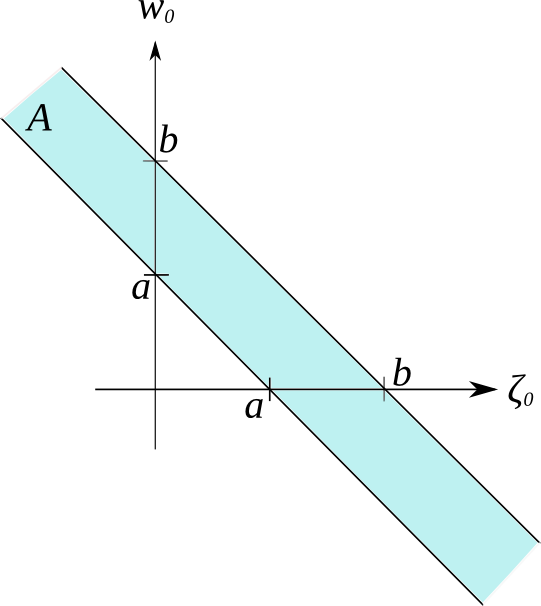
\includegraphics[width=.3\textwidth]{images/02iid}
\caption{Distribution over $A$.}
\label{fig:02iid}
\end{figure}% chktex 17
